\documentclass{ximera}

\graphicspath{{./}{thePythagoreanTheorem/}{deMoivreSavesTheDay/}{complexNumbersFromDifferentAngles/}}

\usepackage{tikz}
\usepackage{tkz-euclide}
\usetkzobj{all}
\tikzstyle geometryDiagrams=[ultra thick,color=blue!50!black]
\newcommand{\tri}{\triangle}
\renewcommand{\l}{\ell}
\renewcommand{\P}{\mathcal{P}}
\newcommand{\R}{\mathbb{R}}
\newcommand{\Q}{\mathbb{Q}}

\newcommand{\Z}{\mathbb Z}

\renewcommand{\vec}{\mathbf}
\renewcommand{\d}{\,d}



%% Egyptian symbols

\usepackage{multido}
\newcommand{\egmil}[1]{\multido{\i=1+1}{#1}{
\includegraphics[scale=.1]{egyptian/egypt_person.pdf}\hspace{0.5mm}}}
\newcommand{\eghuntho}[1]{\multido{\i=1+1}{#1}{
\includegraphics[scale=.1]{egyptian/egypt_fish.pdf}\hspace{0.5mm}}}
\newcommand{\egtentho}[1]{\multido{\i=1+1}{#1}{
\includegraphics[scale=.1]{egyptian/egypt_finger.pdf}\hspace{0.5mm}}}
\newcommand{\egtho}[1]{\multido{\i=1+1}{#1}{
\includegraphics[scale=.1]{egyptian/egypt_lotus.pdf}\hspace{0.5mm}}}
\newcommand{\eghun}[1]{\multido{\i=1+1}{#1}{
\includegraphics[scale=.1]{egyptian/egypt_scroll.pdf}\hspace{0.5mm}}}
\newcommand{\egten}[1]{\multido{\i=1+1}{#1}{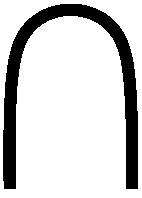
\includegraphics[scale=.1]{egyptian/egypt_heel.pdf}\hspace{0.5mm}}}
\newcommand{\egone}[1]{\multido{\i=1+1}{#1}{
\includegraphics[scale=.1]{egyptian/egypt_stroke.pdf}\hspace{0.5mm}}}
\newcommand{\egyptify}[7]{
 \multido{\i=1+1}{#1}{
\includegraphics[scale=.1]{egyptian/egypt_person.pdf}\hspace{0.5mm}}
 \multido{\i=1+1}{#2}{
\includegraphics[scale=.1]{egyptian/egypt_fish.pdf}\hspace{0.5mm}}
 \multido{\i=1+1}{#3}{
\includegraphics[scale=.1]{egyptian/egypt_finger.pdf}\hspace{0.5mm}}
 \multido{\i=1+1}{#4}{
\includegraphics[scale=.1]{egyptian/egypt_lotus.pdf}\hspace{0.5mm}}
 \multido{\i=1+1}{#5}{
\includegraphics[scale=.1]{egyptian/egypt_scroll.pdf}\hspace{0.5mm}}
 \multido{\i=1+1}{#6}{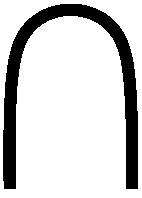
\includegraphics[scale=.1]{egyptian/egypt_heel.pdf}\hspace{0.5mm}}
 \multido{\i=1+1}{#7}{
\includegraphics[scale=.1]{egyptian/egypt_stroke.pdf}\hspace{0.5mm}}
 \hspace{.5mm}
}




\title{The foundations of geometry}
\begin{document}
\begin{abstract}
Now we discuss Hilbert's axioms for plane geometry.
\end{abstract}
\maketitle

In 1889 David Hilbert suggested the following axioms for plane geometry:

\paragraph{I. Incidence}
\begin{enumerate}
\item For every two points $A$ and $B$ there exists a line a that
  contains them both. We write $AB = a$ or $BA = a$.

\item For every two points there exists no more than one line that
  contains them both; consequently, if $AB = a$ and $AC = a$, where
  $B\ne C$, then also $BC = a$.

\item There exist at least two points on a line. There exist at least three
points that do not lie on a line.

\item For every three points $A$, $B$, $C$ not situated on the same
  line there exists a plane $\alpha$ that contains all of them. For
  every plane there exists a point which lies on it. We write $ABC =
  \alpha$.

\item For every three points $A$, $B$, $C$ which do not lie in the
  same line, there exists no more than one plane that contains them
  all.

\item If two points $A$, $B$ of a line $a$ lie in a plane $\alpha$,
  then every point of $a$ lies in $\alpha$.

\item If two planes $\alpha$, $\beta$ have a point $A$ in common, then
  they have at least a second point $B$ in common.

\item There exist at least four points not lying in a plane.
\end{enumerate}

\paragraph{II. Order}

\begin{enumerate}

\item If a point $B$ lies between points $A$ and $C$, $B$ is also
  between $C$ and $A$, and there exists a line containing the distinct
  points $A$, $B$, $C$.

\item If $A$ and $C$ are two points of a line, then there exists at
  least one point $B$ lying between $A$ and $C$.

\item Of any three points situated on a line, there is no more than
  one which lies between the other two.

\item Pasch's Axiom: Let $A$, $B$, $C$ be three points not lying in the same
  line and let $a$ be a line lying in the plane $ABC$ and not passing
  through any of the points $A$, $B$, $C$. Then, if the line $a$ passes
  through a point of the segment $AB$, it will also pass through either
  a point of the segment $BC$ or a point of the segment $AC$.
\end{enumerate}

\paragraph{III. Congruence}
\begin{enumerate}

\item If $A$, $B$ are two points on a line $a$, and if $A'$ is a point upon
  the same or another line $a'$, then, upon a given side of $A'$ on the
  straight line $a'$, we can always find a point $B'$ so that the segment
  $AB$ is congruent to the segment $A'B'$. We indicate this relation by
  writing $AB \cong A' B'$. Every segment is congruent to itself; that is,
  we always have $AB\cong AB$.

\item If a segment $AB$ is congruent to the segment $A'B'$ and also to the
  segment $A''B''$, then the segment $A'B'$ is congruent to the segment
  $A''B''$; that is, if $AB \cong A'B'$ and $AB \cong A''B''$, then $A'B'\cong A''B''$.

\item Let $AB$ and $BC$ be two segments of a line a which have no
  points in common aside from the point $B$, and, furthermore, let
  $A'B'$ and $B'C'$ be two segments of the same or of another line
  $a'$ having, likewise, no point other than $B'$ in common. Then, if
  $AB \cong A'B'$ and $BC \cong B'C'$, we have $AC \cong A'C'$.

\item Let an angle $\angle (h,k)$ be given in the plane $\alpha$ and let a
  line $a'$ be given in a plane $\alpha'$. Suppose also that, in the plane
  $\alpha'$, a definite side of the straight line $a'$ be assigned. Denote
  by $h'$ a ray of the straight line $a'$ emanating from a point $O'$ of
  this line. Then in the plane $\alpha'$ there is one and only one ray
  $k'$ such that the angle $\angle (h, k)$, or $\angle (k, h)$, is congruent
  to the angle $\angle (h', k')$ and at the same time all interior
  points of the angle $\angle (h', k')$ lie upon the given side of
  $a'$. We express this relation by means of the notation $\angle (h, k)
  \cong \angle (h', k')$.

\item If the angle $\angle (h, k)$ is congruent to the angle $\angle
  (h', k')$ and to the angle $\angle (h'', k'')$, then the angle
  $\angle (h', k')$ is congruent to the angle $\angle (h'', k'')$;
  that is to say, if $\angle (h, k) \cong \angle (h', k')$ and $\angle
  (h, k) \cong \angle (h'', k'')$, then $\angle (h', k') \cong \angle
  (h'', k'')$.

\item If, in the two triangles $ABC$ and $A'B'C'$ the congruences $AB
  \cong A'B'$, $AC \cong A'C'$, $\angle BAC \cong \angle B'A'C'$ hold,
  then the congruence $\angle ABC \cong \angle A'B'C'$ holds (and, by a
  change of notation, it follows that $\angle ACB \cong \angle A'C'B'$
  also holds).
\end{enumerate}

\paragraph{IV. Parallels}

\begin{enumerate}

\item (Euclid's Axiom): Let $a$ be any line and $A$ a point not on
  it. Then there is at most one line in the plane, determined by $a$ and
  $A$, that passes through $A$ and does not intersect $a$.
\end{enumerate}

\paragraph{V. Continuity}

\begin{enumerate}
\item Axiom of Archimedes. If $AB$ and $CD$ are any segments then there
  exists a number $n$ such that $n$ segments $CD$ constructed contiguously
  from $A$, along the ray from $A$ through $B$, will pass beyond the point
  $B$.

\item Axiom of line completeness. An extension of a set of points on a
  line with its order and congruence relations that would preserve the
  relations existing among the original elements as well as the
  fundamental properties of line order and congruence that follows
  from Axioms I-III and from V-1 is impossible.
\end{enumerate}


\begin{exploration}
Draw pictures illustrating what these axioms are saying.
\end{exploration}


\begin{question}
If you recall, Euclid only had 5 axioms. What were they?
\end{question}

\begin{question}
How many axioms is Hilbert suggesting? Why did Hilbert suggest so many more axioms than Euclid? 
\end{question}


\end{document}
